\documentclass[a4paper,10pt]{article}
\usepackage[T1]{fontenc}
\usepackage[utf8]{inputenc}
\usepackage[english]{babel}
\usepackage{lmodern}
\usepackage[top=1.4cm,bottom=1.6cm,left=1.8cm,right=1.8cm]{geometry}
\usepackage{titlesec,enumitem,xcolor,graphicx,lastpage,fancyhdr}
\usepackage{fontawesome5}
\usepackage[hidelinks]{hyperref}

\definecolor{accent}{RGB}{0, 70, 140}
\hypersetup{colorlinks=true,urlcolor=accent,linkcolor=accent}
\pagestyle{fancy}\fancyhf{}\renewcommand{\headrulewidth}{0pt}
\fancyfoot[C]{\small\color{gray}Page \thepage\ of \pageref{LastPage}}
\setlength{\parindent}{0pt}
\titleformat{\section}{\large\bfseries\color{accent}}{}{0em}{}[\vspace{-0.7em}\rule{\textwidth}{0.5pt}]
\titlespacing{\section}{0pt}{7pt}{4pt}

\newcommand{\role}[4]{%
 \vspace{2pt}\noindent
 \begin{minipage}[t]{0.70\textwidth}\raggedright\textbf{#1} \textbullet\ \textit{#3}\end{minipage}%
 \hfill
 \begin{minipage}[t]{0.28\textwidth}\raggedleft\footnotesize\color{gray}#2 \textbullet\ #4\end{minipage}%
 \vspace{1pt}%
}
\setlist[itemize]{leftmargin=1.2em, itemsep=1.5pt, topsep=2pt, parsep=0pt}

\begin{document}

% ================= HEADER (HEADLINE is tailored) =================
\begin{minipage}[c]{0.80\textwidth}
 {\Huge\bfseries Prabhavit Gupta}\\[3pt]
 {\color{accent}\large Forward-Deployed Engineer: LLM Data Workflows, Production Logic \& Integrations}\\[6pt]
 {\footnotesize +39 351 610 7807 ~$\vert$~
 \href{mailto:prabhavitg@gmail.com}{prabhavitg@gmail.com} ~$\vert$~
 \href{https://www.linkedin.com/in/prabhavit/}{linkedin.com/in/prabhavit} ~$\vert$~
 \href{https://github.com/prab-gupta}{github.com/prab-gupta} ~$\vert$~
 Venice, Italy}
\end{minipage}\hfill
\begin{minipage}[c]{0.18\textwidth}
 \raggedleft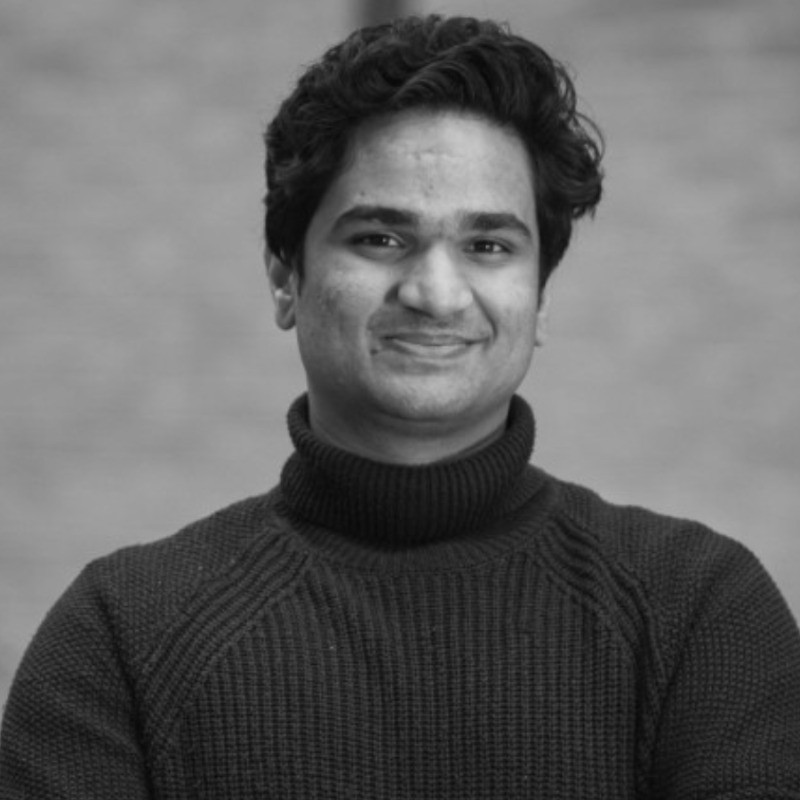
\includegraphics[width=2.0cm]{photo.jpg}
\end{minipage}
\vspace{-2pt}

% ================= SUMMARY (tailored) =================
\section{Summary}
AI and automation engineer with about three years of experience building LLM workflows, data ingestion pipelines, and integrations grounded in how business teams operate. At FlowSpace I built an LLM document ingestion pipeline (900+ listings extracted from PDFs, spreadsheets, and web pages), customer-facing AI agents answering over live platform data with human-in-the-loop escalation, and end-to-end API integrations connecting CRMs and booking systems. Experienced modeling business logic, transforming messy mid-market data exports into structured formats, and deploying reliable production systems with TypeScript, Python, SQL, and Claude Code. Based in Venice, ready to relocate immediately to Munich.

% ================= EXPERIENCE (frozen) =================
\section{Experience}

\role{\href{https://flowspace.co}{FlowSpace.co}}{Mar 2024 - Aug 2026}{Lead Developer (Full-time, Freelance)}{London, UK (remote)}
\begin{itemize}
 \item Built an AI listing bot with a human in the loop: it takes a brochure in any format (PDF, web page, photo or spreadsheet), drafts the full listing with an LLM, and pushes it to the backend after review. 900+ listings drafted.
 \item Streamlined customer support with AI agents that answer queries against live platform data and escalate to a person on low confidence.
 \item Integrated the OfficeRnD and Nexudus APIs for automated bookings, and built CRM lead-capture integration and GTM automations (sales funnel, lead enrichment, outbound) with n8n.
 \item Led the migration off a legacy stack to a coded Next.js and Laravel product: mapped the data model, chose the migration path per entity (API or CSV) and drove the cutover. Scaled the platform from 2,000 to 4,500+ users.
 \item Documented product and business logic with the developer team, coordinated between the internal team and an external agency, and built a commute-time calculator tool for companies.
 \item \textit{Tools: Claude Code, n8n, Playwright, Postman, Laravel, TypeScript, Supabase, GitHub, Jira, ClickUp, Miro, Google Analytics, Microsoft Clarity}
\end{itemize}

\role{\href{https://smarturlink.com/}{Urlink}}{Apr 2025 - Jul 2025}{Project Manager and AI-Assisted Developer (Freelance)}{Barcelona, Spain}
\begin{itemize}
 \item Used AI to build the platform and its logic, implemented AI-made UIs, and built automations to client requirements.
 \item \textit{Tools: GitHub, Netlify, Supabase, bolt.new}
\end{itemize}

\role{\href{https://ultrastrategy.com}{UltraStrategy.com}}{Dec 2024 - May 2025}{Automation Developer (Collaborator)}{France}
\begin{itemize}
 \item Built a CV-parsing tool with n8n and Eden AI (LLM data extraction) and a platform for different user profiles.
 \item \textit{Tools: n8n, Eden AI}
\end{itemize}

\role{\href{https://www.qomodo.me/}{Qomodo}}{2024 - Jan 2025}{AI and Low-Code Developer (Collaborator)}{Milan, Italy}
\begin{itemize}
 \item Built a dashboard for companies to manage their branches and implemented Figma designs.
\end{itemize}

\role{\href{https://get2germany.com}{Get2Germany.com}}{Jan 2024 - May 2024}{Lead Developer and Automation Specialist (Part-time)}{Berlin, Germany}
\begin{itemize}
 \item Integrated Google APIs for platform tracking, built the platform and optimized the database, and developed AI-based automation tools for finding courses, internships and jobs.
 \item \textit{Tools: n8n, Figma, Trello, Google APIs}
\end{itemize}

\role{\href{https://clubee.com}{Clubee.com}}{Sep 2023 - Aug 2024}{Low-Code Developer and Quality Assurance (Full-time, Freelance)}{Foetz, Luxembourg}
\begin{itemize}
 \item Integrated the Clubee API across the whole frontend, ran unit testing and QA on new features, and built tools for domain integration, a shop and a federation dashboard.
 \item \textit{Tools: Figma, GitHub, Postman, REST APIs}
\end{itemize}

\role{\href{https://tractionboard.co}{Tractionboard.co}}{Aug 2023 - Oct 2023}{Low-Code Developer (Internship)}{Utrecht, Netherlands}
\begin{itemize}
 \item Integrated ChatGPT/OpenAI and Sendgrid, built responsive designs, debugged features and implemented Google Ads 4.
 \item \textit{Tools: Figma, Sendgrid, ChatGPT}
\end{itemize}

% ================= EDUCATION (frozen) =================
\section{Education}
\role{Ca' Foscari University of Venice}{Oct 2020 - Jun 2024}{Bachelor's in Philosophy, International Studies \& Economics, Minor in Entrepreneurship}{Venice, Italy}

% ================= CERTIFICATIONS (frozen) =================
\section{Certifications}
Microsoft Copilot Studio Agent Academy \textbullet\ Microsoft: Introduction to building AI agents \textbullet\ Microsoft Power Automate \textbullet\ Tray.AI Build Practitioner (Sep 2024) \textbullet\ Tray.AI Build Foundations

% ================= ADDITIONAL INFORMATION (frozen) =================
\section{Additional Information}
\begin{itemize}
 \item \textbf{Work authorization:} European Long Term Residence Permit (Italy), no sponsorship needed in the EU. Available immediately.
 \item \textbf{Languages:} Hindi (native), English (professional), Italian (beginner).
\end{itemize}

% ================= CORE SKILLS (tailored, at the bottom) =================
\section{Core Skills}
\begin{itemize}
 \item \textbf{LLM workflows and agents:} AI agents, prompts and context engineering, tool use and function calling, RAG, structured data extraction, human-in-the-loop review, confidence thresholds and escalation, Claude and OpenAI APIs, Claude Code
 \item \textbf{Data, SQL and logic modeling:} SQL querying, relational data modeling, data transformation, JSON, CSV and spreadsheet normalization, ERP and CRM data handling, Supabase, PostgreSQL
 \item \textbf{Integration and APIs:} REST APIs, authentication (OAuth, API keys), webhooks, data pipelines, third-party integrations (OfficeRnD, Nexudus, Google APIs, Sendgrid), Postman, n8n
 \item \textbf{Customer and production delivery:} Direct customer collaboration from Day 1, understanding operational bottlenecks, requirements discovery, production deployment, troubleshooting, technical documentation
\end{itemize}

\end{document}
